\subsection{Exam: 2022. 05. 30., Exercise 5}

\lineparagraph{Exercise}

Pairwise distinct keys are stored in a binary search tree. It is known that
node $x$ of the tree has two children. How many children the node $y$ can have,
whose key is the successor of the key of $x$ in the ordering of the keys?

\lineparagraph{Solution}

\begin{itemize}
    \item Successor means that $x<y$ and $x$ is immediately followed by $y$, with nothing between the two.
    \item Since $x$ and $y$ immediately follow each other, one of them has to be the ancestor of the other one. If they are not ancestor of each other, then if we take their first common ancestor, e.g. $k$, $x$ and $y$ will be on different sides of $k$. Which would mean that $k$ comes between $x$ and $y$ in the order, so they couldn't be successors.
\end{itemize}

\begin{center}
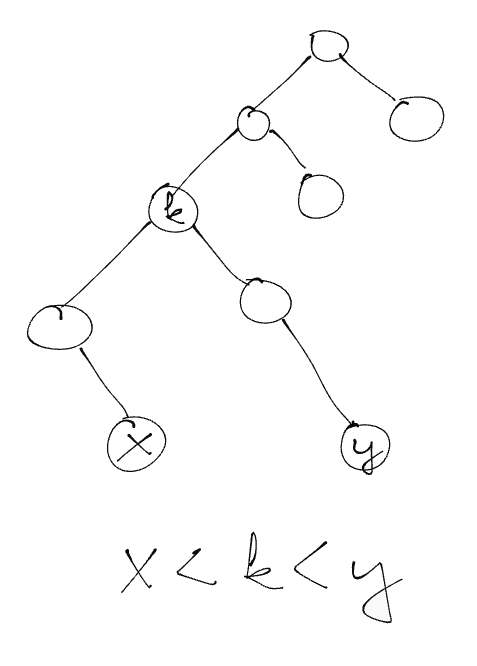
\includegraphics[width=0.4\linewidth]{./exams/2022_05_30/05/common_parent.png}
\end{center}

\begin{itemize}
    \item Either $x$ is an ancestor to $y$ or $y$ is an ancestor to $x$.
    \item If $y$ is the ancestor of $x$, then:
\end{itemize}

\begin{center}
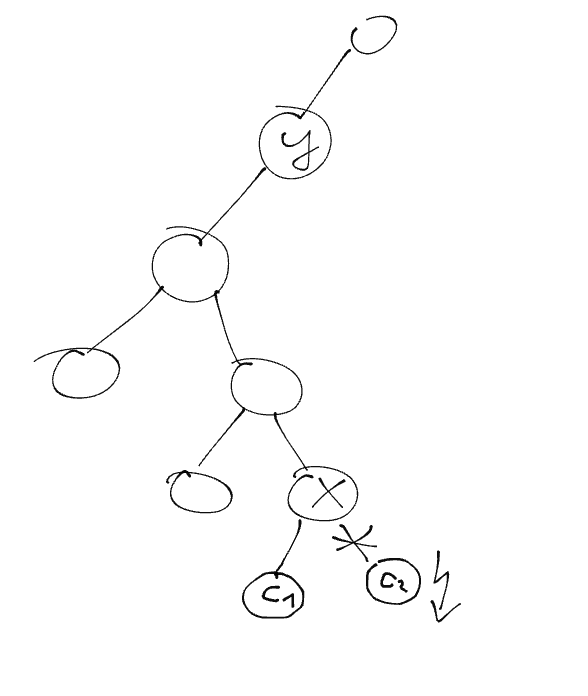
\includegraphics[width=0.4\linewidth]{./exams/2022_05_30/05/yancestor.png}
\end{center}

\begin{itemize}
    \item Then $x$ cannot have a right child $c_2$, since that would come between $x$ and $y$: $x<c_2<y$. But the task says that $x$ has two children, so this case cannot happen.
    \item This means that $x$ is the ancestor of $y$:
\end{itemize}

\begin{center}
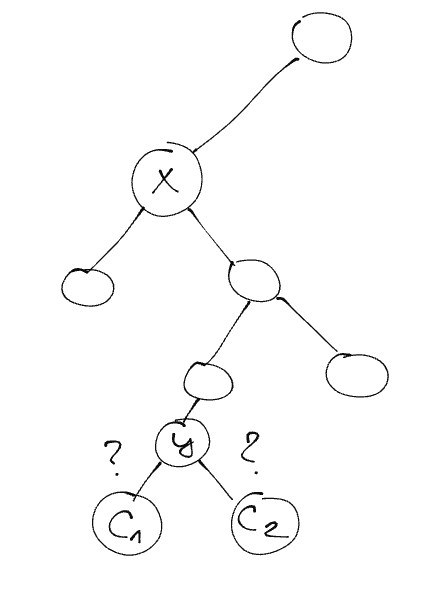
\includegraphics[width=0.4\linewidth]{./exams/2022_05_30/05/xancestor.png}
\end{center}

\begin{itemize}
    \item $y$ must be on the righthand side of $x$, since $x<y$, however it must be the leftmost child in that substree, since nothing can come between $x$ and $y$.
    \item $y$ cannot have a lefthand side child $c_1$, since that would come between $x$ and $y$, $x<c_1<y$, which would make $x$ and $y$ not be successors.
    \item $y$ can have $0$ children or $1$ child (the right child), but not $2$ children.
\end{itemize}